\subsubsection{Campo debole}
Si considera la metrica D-dimensionale $g_{\mu\nu}$ nell'approssimazione di campo debole.
Le Vielbein possono essere scritte come \( V^a = (\delta^a_\mu + \frac{1}{2} h^a_\mu) \dx^\mu \): si verifica infatti che, al primo ordine in $|h_{\mu\nu}|$, 
\[ \eta_{ab} V^aV^b = g_{\mu\nu}\dx^\mu \dx^\nu \]
Si verifica immediatamente che 
\[ V^\mu_a = (\delta^\mu_a - \frac{1}{2} h^\mu_a) \]
pertanto si pu\`o usare la formula
\[ \omega_{abc} = V^\mu_a V^\nu_b \partial_\mu V^c_\nu - [cab] + [bca] \]
che, considerando di secondo ordine termini del tipo $(\partial h)h$, porta al primo ordine a 
\[ \omega_{abc} = \frac{1}{2} [ \partial{[b} h_{c]a} - [abc] + [cab] \]
\[ \omega_{ab} = \frac{1}{2} \partial_{[b} h_{a]c} V^c \]
Siccome si trascurano termini del tipo $(\partial h)(\partial h)$,
\[ R_{ab} = \de \omega_{ab} = -\frac{1}{2} \partial_i \partial_{[a} h_{b]j} V^i \wedge V^j \]

Lo stesso calcolo si pu\`o fare con i simboli di Christoffel:
\[ \Gamma ^\sigma_{\mu\nu} = \frac{1}{2} g^{\rho\sigma}(\partial_\mu g_{\nu\rho} + [\nu\rho\mu] - [\rho\mu\nu]) = \frac{1}{2}(\partial_\mu h^\sigma_\mu + \partial_\nu h^\sigma_\mu - \partial^\sigma h_{\mu\nu} ) \]
e
\[ R_{\mu\nu} = -\partial_{\alpha} \partial_{[\mu} h_{\nu]\beta} \dx^\alpha \dx^\beta \]

Il tensore di Ricci \`e
\[ Ric_{ab} = - \frac{1}{2} \partial^2  h_{ab} + \frac{1}{2} \partial_\nu \partial^\mu h^b_\mu 
              + \frac{1}{2} \partial_\mu \partial^b h^\mu_\nu - \frac{1}{2} \partial_\nu \partial^b h  \]
che con la gauge 
\[ \partial^a \bar{h}_{ab} = 0  \;\;\; ; \;\;\; \bar{h}_{ab} = h_{ab} - \frac{1}{2} \eta_{ab} h \]
diventa
\[ Ric_{ab} = - \frac{1}{2} \partial^2  h_{ab} \]
da cui il tensore di Einstein \`e immediatamente
\[ G_{\mu\nu} = -\frac{1}{2} \partial^2 \bar{h}_{\mu\nu} \]

\subsubsection{Gauge "di Lorenz"}
Presa una variazione
\[ x'^\mu = x^\mu +\epsilon^\mu(x) \;\;\;\rightarrow \;\;\; \dx'^\mu = \dx^\mu + \partial_\nu \epsilon^\mu \dx^\nu \]
e considerando che la metrica deve restare invariata
\[ g_{\mu\nu}(x)\dx^\mu\dx^\nu = g'_{\mu\nu}(x')\dx'^\mu\dx'^\nu \]
Il primo membro \`e semplicemente \( \eta_{\mu\nu} \dx^\mu\dx^\nu + h_{\mu\nu} \dx^\mu\dx^\nu \), mentre il secondo pu\`o essere espanso al primo ordine come
\[ (g'_{\mu\nu}(x)+\partial_\rho g'_{\mu\nu}(x) \epsilon^\rho)  \dx'^\mu\dx'^\nu = (\eta_{\mu\nu} + h'_{\mu\nu}(x) + \partial_\rho h'_{\mu\nu} \epsilon^\rho) \dx'^\mu\dx'^\nu \]
Quindi uguagliando le due metriche (trascurando i termini $h\epsilon$ o $\partial h\epsilon$)
\[ h_{\mu\nu} \dx^\mu\dx^\nu = \eta_{\mu\nu} \partial_\rho \epsilon^\mu \dx^\rho \dx^\nu + 
                               \eta_{\mu\nu} \partial_\rho \epsilon^\nu \dx^\mu \dx^\rho + 
			       h'_{\mu\nu}(x) \dx^\mu\dx^\nu \]
da cui
\[ h'_{\mu\nu} = h_{\mu\nu} -  \partial_\mu \epsilon_\nu - \partial_\nu \epsilon^\mu \;\;\;;\;\;\;
	\partial^\mu h'_{\mu\nu} = \partial^\mu h_{\mu\nu} - \partial^2 \epsilon_\nu - \partial_\mu \partial_\nu \epsilon^\mu \;\;\;;\;\;\;
	h' = h - 2\partial^\mu \epsilon_\mu \]
e imponendo la gauge
\[ \partial^\mu \bar{h}_{\mu\nu} - \partial^2\epsilon_\nu =0 \]

Per il potenziale Elettromagnetico, invece, 
\[ A'_\mu = A_\mu + \partial_\mu \epsilon \]
e nella gauge di Lorenz
\[ \partial^\mu A_\mu - \partial^2 \epsilon = 0 \]


\subsubsection{Equazioni di Einstein}
In definitiva l'equazione di Einstein diventa
\[ \frac{8\pi G}{c^4} T_{\mu\nu} = G_{\mu\nu} = -\frac{1}{2} \partial^2 \bar{h}_{\mu\nu} \]
\begin{equation} \label{eq:einst_lin}
	\partial^2 \bar{h}_{\mu\nu} = -\frac{16\pi G}{c^4} T_{\mu\nu} 
\end{equation}

\subsubsection{Funzione di Green}
La funzione di Green del D'Alambertiano, valutata nella sua trasformata di Fourier, risulta essere \( \tilde{G} =- 1/k^2 \). Dovendo integrare questa espressione in $k^0$, si nota subito che ha due poli per \( k^0 = |\vec{k}| \), per cui sar\`a necessaria una prescrizione $i\epsilon$, concretizzata in un cambio di variabile \( k^0 -> k^0 \pm i\epsilon \). La richiesta di causalit\`a permette di fissarne il segno, in quanto corrisponde alla richiesta che la funzione sia nulla per \( x^0 < 0\):  infatti, usando il lemma di Jordan, l'integrale in questo intervallo si annulla chiudendo la circonferenza "sopra" l'asse reale; ma, richiedendo che sia nullo, esso non deve contenere i poli, pertanto si ha una situazione come in \ref{figure:green}.


\begin{figure}[htbp]
 \centering
 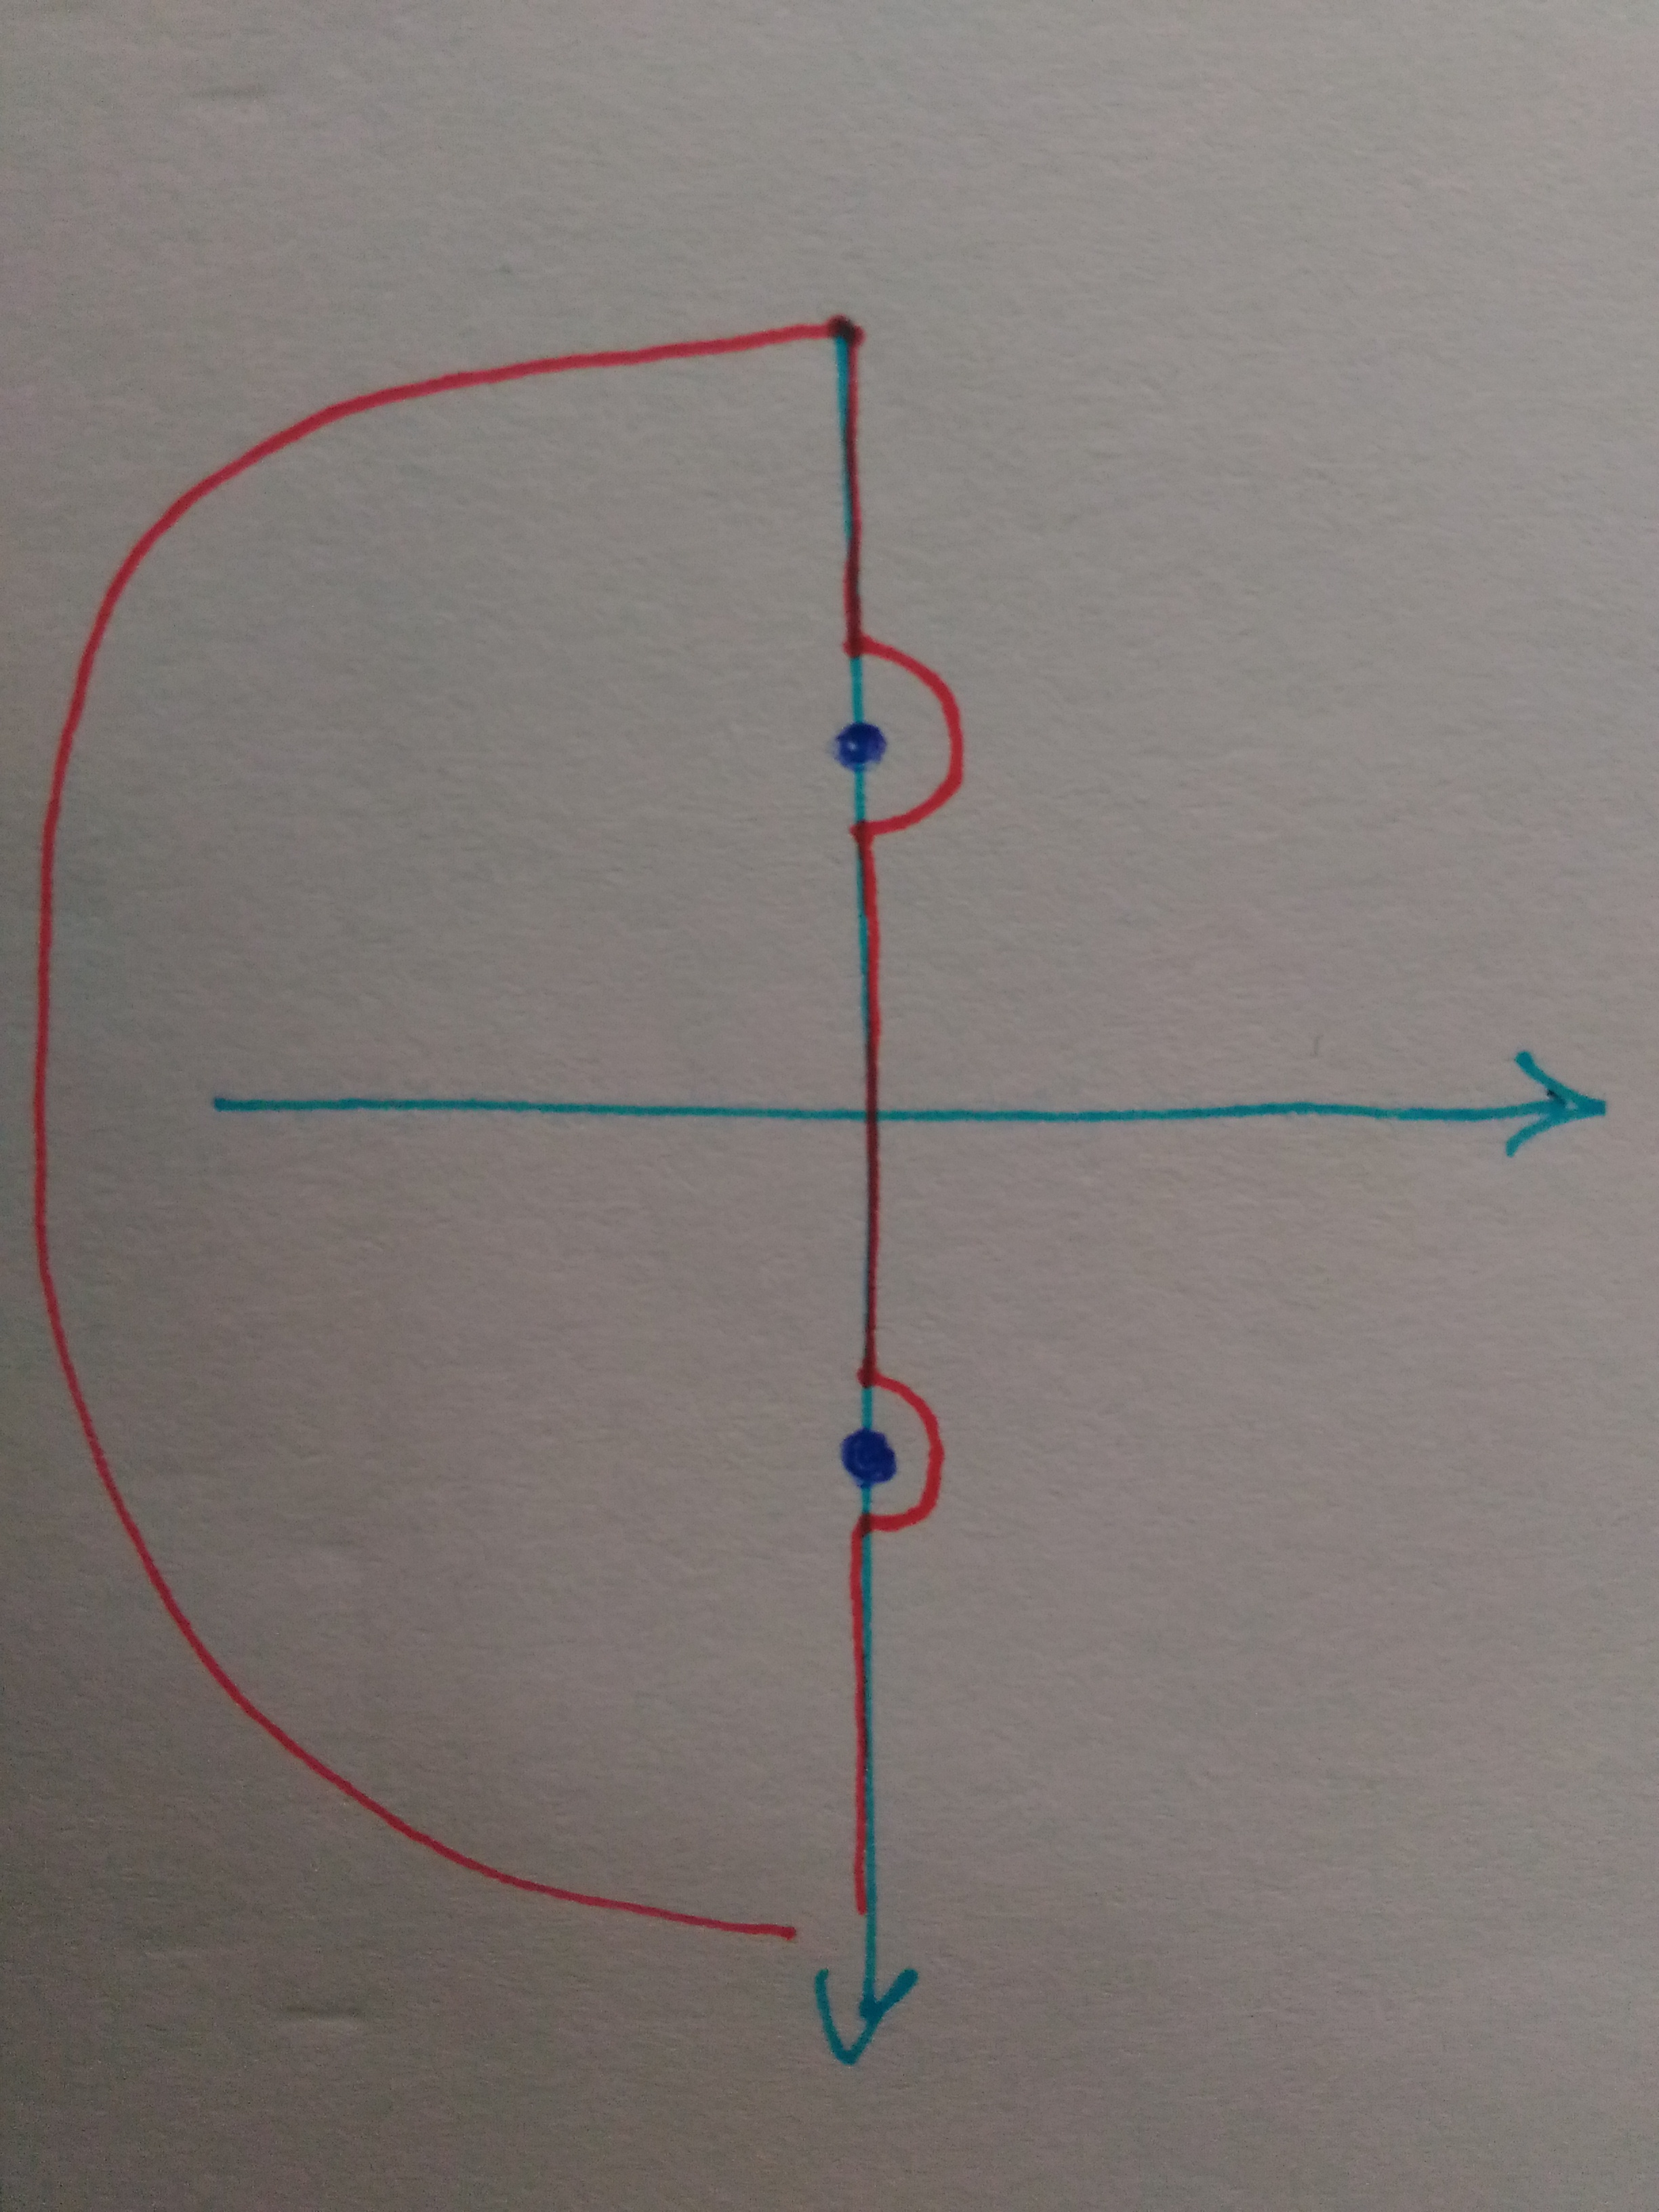
\includegraphics[angle=90, width=0.35\textwidth]{images/foglio5_circuito}
	\caption*{}
 \label{figure:green}
\end{figure}

L'integrale risulta quindi
\[ G_R = \int \frac{\de ^4k}{(2\pi)^4} \frac{e^{ik_\mu x^\mu}}{ (k^0+i\epsilon)^2 - \vec{k}^2 } \]
che diventa col teorema dei residui, in coordinate sferiche
\[ G_R = -\frac{1}{(2\pi)^4} \int \de \phi \; \de \cos\theta \;\de k \;\; k^2 e^{ ik|x|\cos\theta} \frac{2\pi i}{2k} \left[e^{-ikx^0} - e^{ikx^0}\right] \theta(x^0)    \]
\[ G_R = \frac{1}{(2\pi)^2} \frac{1}{2|x|} \int \de k \left( e^{ik|x|} - e^{-ik|x|}\right) \left(e^{-ikx^0} - e^{ikx^0} \right)\theta(x^0)  \]
\[ G_R = \frac{2}{(2\pi)^2 |x|} \int \de k \sin(k|x|) \sin(kx^0) \theta(x^0) \]
Alternativamente, sviluppando i prodotti di esponenziali e cambiando variabile per gli esponenti con segno negativo, utilizzando infine la forma integrale della delta di Dirac \( 2\pi\delta(x) = \int \de k e^{ikx} \) si trova
\[ G_R = -\frac{1}{4\pi|\vec{x}|}\delta{x^0-|\vec{x}|} \]
dove la $\theta$ \`e sottintesa dalla $\delta$.

\subsubsection{Polvere}
Per le propriet\`a della funzione di Green, la \ref{eq:einst_lin} ha soluzione
\[ \bar{h}_{\mu\nu} (x^0,\vec{x}) = \int G_R(x-y) \left[ -\frac{16\pi G}{c^4} T_{\mu\nu}(y) \right] 
		= \frac{4G}{c^4} \int \de ^4y \frac{ T_{\mu\nu}(y) \delta(x^0-y^0-|\vec{x}- \vec{y}|}{|\vec{x}-\vec{y}|} \]
\[ \bar{h}_{\mu\nu} (x^0,\vec{x}) = \frac{4G}{c^4} \int \de ^3y \frac{ T_{\mu\nu}(x^0-|\vec{x}-\vec{y}|, \vec{y})}{|\vec{x}-\vec{y}|} \]

Preso il tensore energia-impulso della polvere
\[ T_{\mu\nu} = (c^2 \rho +p)u_\mu u_\nu + g_{\mu\nu} p \]
nelle condizioni 
\[ u^\mu = (1,\vec{0}) \;\;\; ; \;\;\; |p| << c^2\rho \;\;\; ; \;\;\; \rho = \rho(\vec{y}) \]
Se la materia \`e confinata in un raggio $|\vec{y}_M|$ e il campo viene valutato a distanze molto maggiori di questo raggio, si pu\`o sviluppare
\[ \frac{1}{|\vec{x}-\vec{y}|} \sim \frac{1}{|\vec{x}|} \]
Il tensore energia-impulso si riduce, nelle condizioni date, a
\[ T_{00} = c^2\rho \;\;\; ; \;\;\; T_{ii} = p  \;\;\; ; \;\;\; T = -T_{00} +3 T_{ii} \sim -T_{00} \]
per cui
\[ h_{00} = \bar{h}_{00} + \frac{1}{2} \eta_{00} h = \frac{4G}{c^4|\vec{x}|} \int \de^3y (c^2\rho - \frac{1}{2}c^2\rho) = \frac{2GM}{c^2|\vec{x}|} \]
\[ h_{ii} = \bar{h}_{ii} + \frac{1}{2} \eta_{ii} h = \frac{4G}{c^4|\vec{x}|} \int \de^3y (p + \frac{1}{2}c^2\rho) \sim \frac{2GM}{c^2|\vec{x}|} \]

quindi la metrica diventa
\[ \de s^2 = -(1-\frac{2GM}{c^2r})c^2\de t^2 + (1+\frac{2GM}{c^2r})(\de \vec{x})^2 \]
da cui si vede che, perch\'e resti valido il limite di campo debole, dev'essere
\[ 2GM << c^2r \;\;\;\rightarrow \;\;\; M<<\frac{c^2R}{2G} \]




\subsubsection{Centro di massa nell'origine}
Si prende il centro di massa nell'origine, con velocit\`a nulla. Si considera \( u^\mu \sim (1,\vec{v}/c) \).
\[ T_{00} = c^2\rho \;\;\; ; \;\;\; T_{0i} \sim c\rho v_i \sim T_{00}/c \;\;\; ; \;\;\; T_{ij} \sim \rho v_i v_j\sim T_{00}/c^2 \]
Usando la conservazione di $T_{\mu\nu}$
\[ \partial_\mu T^{\mu\nu} \rightarrow \partial_k T^{k0} = - \partial_0 T^{00} \]
e quindi 
\[ \int_V \de^3y \partial_kT^{0k} y_iy_j = -\int_V \de^3y \partial_0T^{00} y_iy_j  = -\left[ T^{00}y_iy_j\right|_\Sigma + \int \de^3y c^2 T^{00} (v_iy_j + y_iv_j) \]
\begin{equation} \label{eq:commut}
	\partial_0\rho(\vec{y}) = 0 \Rightarrow \partial_0T^{00} = 0 \Rightarrow \int \de^3y T^{00} (v_iy_j + y_iv_j) =0 
\end{equation}
Dove si \`e trascurato il termine di bordo in quanto \todo

Si sviluppa in multipoli
\[ \frac{1}{|\vec{x}-\vec{y}|} \sim \frac{1}{|\vec{x}|} + y^i \frac{x_i}{|\vec{x}|^3} + \mathcal{O}(r^{-5}) \]
da cui
\[ \bar{h}_{00}(x^0,\vec{x}) = \frac{2GM}{c^2 r} + \mathcal{O}(r^{-5}) \]
usando la condizione di massa centrata nell'origine, per cui \( \int \de^3y\rho(\vec{y})y_i = 0\); i termini $T_{ij}$ si trascurano, essendo di ordine $T_{00}/c^2$; infine
\[ \bar{h}_{0i}(x^0,\vec{x}) \sim \frac{4G}{c^3} \int \de^3y 
	\left[ 
		\frac{\rho(\vec{y})v_i}{|\vec{x}|}     
	      - \frac{\rho(\vec{y})v_iy_j x^j}{|\vec{x}|^3} 
	\right] \] 
Il primo termine si annulla: la condizione di centro di massa fermo implica infatti \( \int \de^3y\rho(\vec{y})v_i = 0\). Per quanto riguarda il secondo, grazie a \ref{eq:commut}, si verifica che
\[ \frac{1}{2} \int \de^3y \rho (v_iy_j - y_iv_j) = \int \de^3y \rho v_iy_j \]
pertanto
\[ \bar{h}_{0i}(x^0,\vec{x}) \sim -\frac{2Gx^j}{c^3|\vec{x}|} \int \de^3y \rho(\vec{y}) (v_iy_j - v_jy_i) + \mathcal{O}(r^{-5})  \]
Per cui la metrica diventa, usando \( J_{ij} = \int \de^3y \rho(|\vec{y}|) (v_iy_j - v_jy_i) \),
\[ \de s^2 = -(1 - \frac{2GM}{c^2 r} ) c^2 \de t^2 + (1+\frac{2GM}{c^2 r} ) (\de\vec{x})^2 + \frac{4G}{c^3r^3}J_{ij}\de x^i c \de t + \mathcal{O}(r^-5) \]
\todo perch\`e h00 = hii? 
\todo trascinamento

